%%%%%%%%%%%%%%%%%%%%%%%%%%%%%%%%%%%%%%%%%
% baposter Landscape Poster
% LaTeX Template
% Version 1.0 (11/06/13)
%
% baposter Class Created by:
% Brian Amberg (baposter@brian-amberg.de)
%
% This template has been downloaded from:
% http://www.LaTeXTemplates.com
%
% License:
% CC BY-NC-SA 3.0 (http://creativecommons.org/licenses/by-nc-sa/3.0/)
%
%%%%%%%%%%%%%%%%%%%%%%%%%%%%%%%%%%%%%%%%%

%----------------------------------------------------------------------------------------
%	PACKAGES AND OTHER DOCUMENT CONFIGURATIONS
%----------------------------------------------------------------------------------------

\documentclass[landscape,a0paper,fontscale=0.285]{baposter} % Adjust the font scale/size here

\usepackage{graphicx} % Required for including images
\graphicspath{{figures/}} % Directory in which figures are stored

\usepackage{amsmath} % For typesetting math
\usepackage{amssymb} % Adds new symbols to be used in math mode

\usepackage{booktabs} % Top and bottom rules for tables
\usepackage{enumitem} % Used to reduce itemize/enumerate spacing
\usepackage{palatino} % Use the Palatino font
\usepackage[font=small,labelfont=bf]{caption} % Required for specifying captions to tables and figures

\usepackage{multicol} % Required for multiple columns
\setlength{\columnsep}{1.5em} % Slightly increase the space between columns
\setlength{\columnseprule}{0mm} % No horizontal rule between columns

\usepackage{tikz} % Required for flow chart
\usetikzlibrary{shapes,arrows} % Tikz libraries required for the flow chart in the template

\newcommand{\compresslist}{ % Define a command to reduce spacing within itemize/enumerate environments, this is used right after \begin{itemize} or \begin{enumerate}
\setlength{\itemsep}{1pt}
\setlength{\parskip}{0pt}
\setlength{\parsep}{0pt}
}

\definecolor{lightblue}{rgb}{0.145,0.6666,1} % Defines the color used for content box headers

\begin{document}

\begin{poster}
{
headerborder=closed, % Adds a border around the header of content boxes
colspacing=1em, % Column spacing
bgColorOne=white, % Background color for the gradient on the left side of the poster
bgColorTwo=white, % Background color for the gradient on the right side of the poster
borderColor=lightblue, % Border color
headerColorOne=black, % Background color for the header in the content boxes (left side)
headerColorTwo=lightblue, % Background color for the header in the content boxes (right side)
headerFontColor=white, % Text color for the header text in the content boxes
boxColorOne=white, % Background color of the content boxes
textborder=roundedleft, % Format of the border around content boxes, can be: none, bars, coils, triangles, rectangle, rounded, roundedsmall, roundedright or faded
eyecatcher=true, % Set to false for ignoring the left logo in the title and move the title left
headerheight=0.1\textheight, % Height of the header
headershape=roundedright, % Specify the rounded corner in the content box headers, can be: rectangle, small-rounded, roundedright, roundedleft or rounded
headerfont=\Large\bf\textsc, % Large, bold and sans serif font in the headers of content boxes
%textfont={\setlength{\parindent}{1.5em}}, % Uncomment for paragraph indentation
linewidth=2pt % Width of the border lines around content boxes
}
%----------------------------------------------------------------------------------------
%	TITLE SECTION 
%----------------------------------------------------------------------------------------
%
{
\includegraphics[height=4em]{loopq.png}} % First university/lab logo on the left
%\caption{taken from \cite{ref:loopq}}
{\bf\textsc{Loop Q PRIZE Qualifying Challenge 2019}\vspace{0.5em}} % Poster title
{\textsc{\{ Michal Ostyk-Narbutt \} \hspace{12pt} Sapienza University of Rome}} % Author names and institution
{
\includegraphics[height=4em]{logo.png}} % Second university/lab logo on the right

%----------------------------------------------------------------------------------------
%	INTRODUCTION
%----------------------------------------------------------------------------------------

\headerbox{Introduction}{name=conclusion,column=0,span=1,row=0}{

\begin{multicols}{2}

The goal of this was to bla bla\\
The goal of this was to bla bla\\
The goal of this was to bla bla\\
The goal of this was to bla bla
%------------------------------------------------

The goal of this was to bla bla\\
The goal of this was to bla bla\\
The goal of this was to bla bla\\
The goal of this was to bla bla


\end{multicols}
}

%----------------------------------------------------------------------------------------
%	OBJECTIVES
%----------------------------------------------------------------------------------------

\headerbox{Methodology}{name=methodology, column=1,span=1,row=0}{

Donec non nisl a \textbf{arcu consequat} varius. Sed suscipit, a cursus luctus. Nulla sit amet elit augue. Curabitur scelerisque mollis dolor, quis blandit lorem condimentum at. Pellentesque sed nibh vel \textbf{dolor} sagittis semper. 

\begin{enumerate}\compresslist
\item Feugiat vitae elit
\item bibendum ante sed lacinia eros in
\item Curabitur scelerisque arcu consequat varius
\end{enumerate}

%\vspace{0.3em} % When there are two boxes, some whitespace may need to be added if the one on the right has more content
}



%----------------------------------------------------------------------------------------
%	DATASET
%----------------------------------------------------------------------------------------

\headerbox{Dataset}{name=dataset,column=0,span=2,row=1, below=methodology}{

\vspace{1em}
\begin{center}
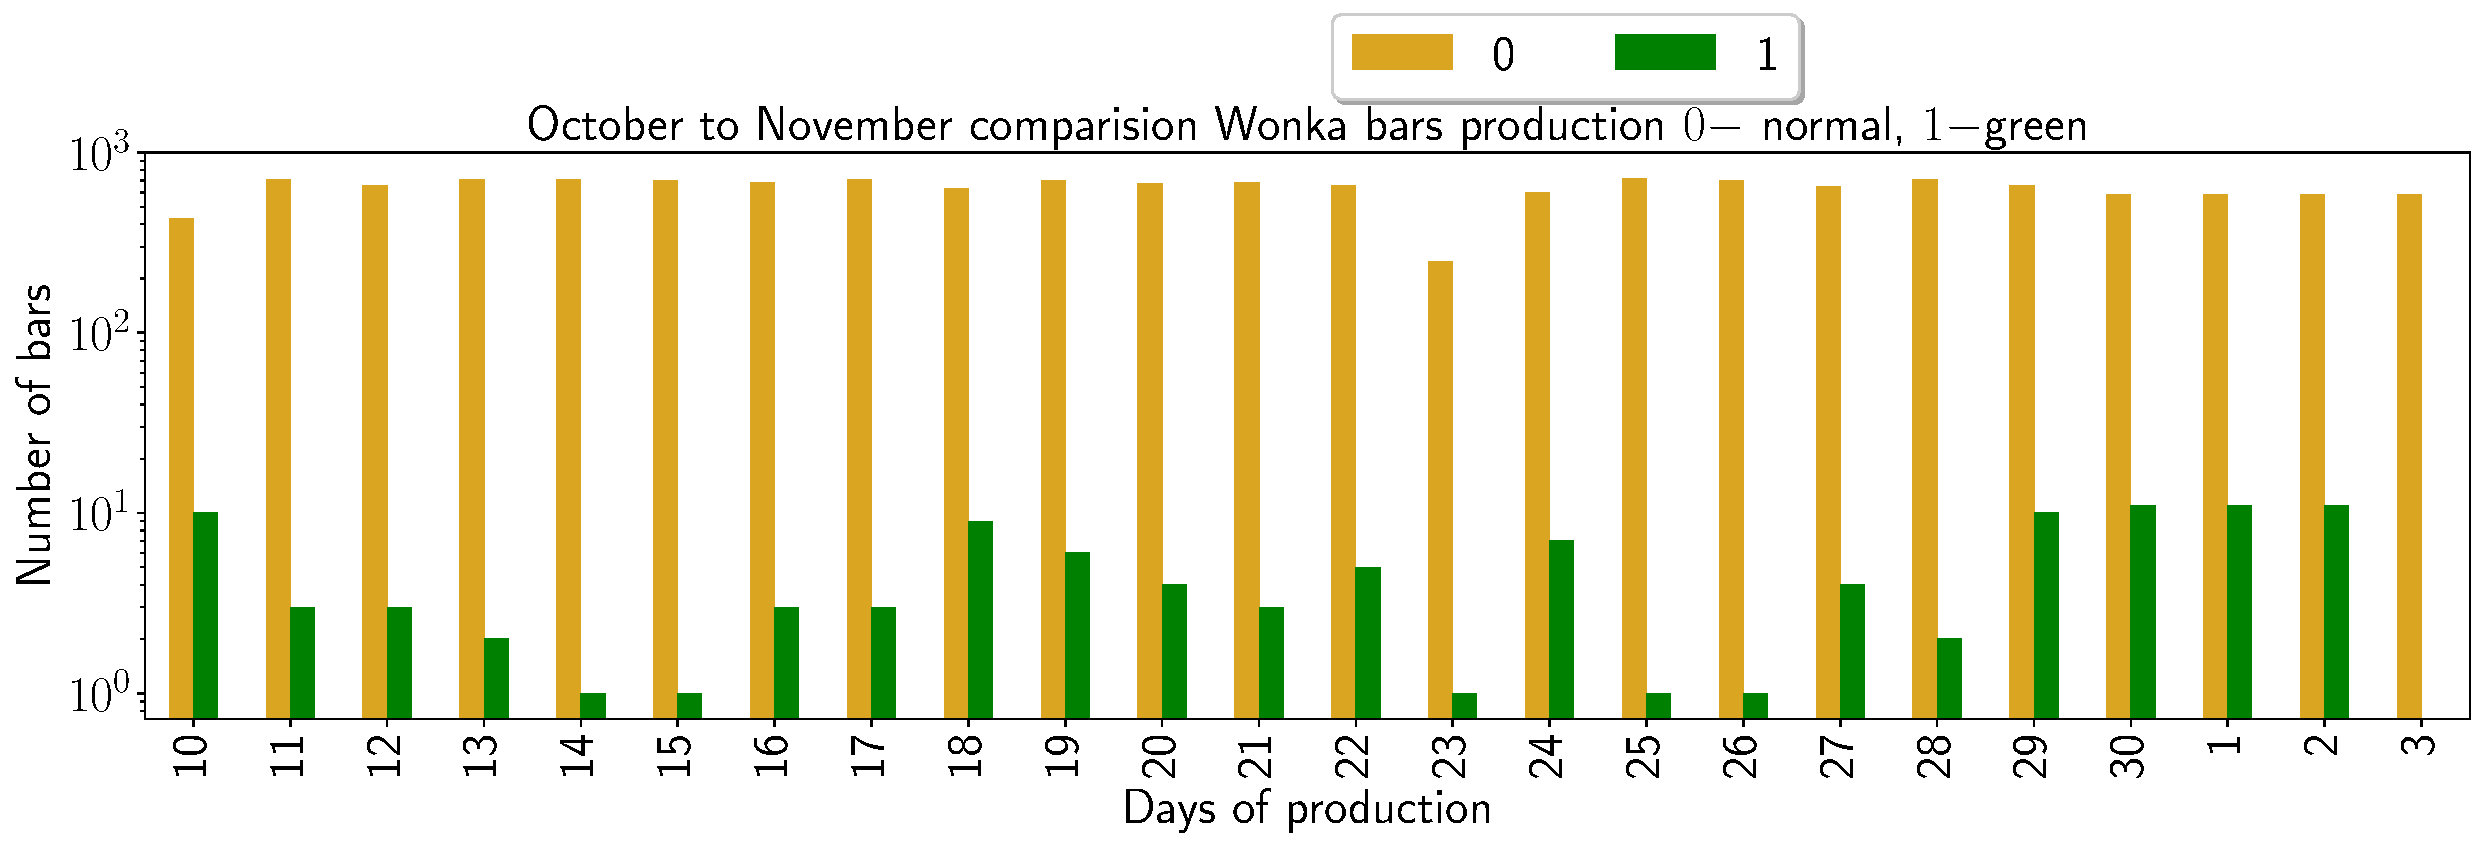
\includegraphics[width=\linewidth]{data_overview.pdf}
\captionof{figure}{Analysis of production of golden (0) and green(1) chocolate bars through the month of October to early November 2018}
\end{center}

%------------------------------------------------

\begin{multicols}{2}


\begin{center}
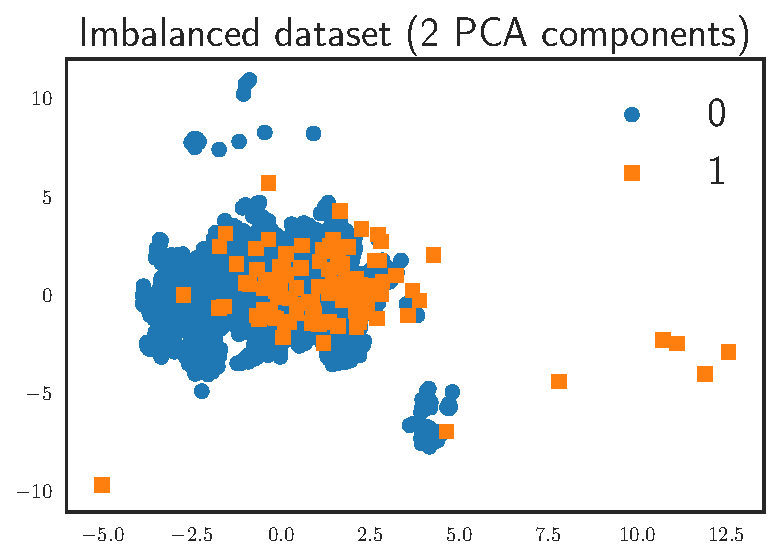
\includegraphics[width=0.8\linewidth]{Imbalanced_dataset_(2_PCA_components)pca.pdf}
\captionof{figure}{Normalised data with applied Principal Comonent Analysis  (PCA) dimensionality reduction. The plot shows that it is extreamly difficult  to distinguish between 0 (gold) and 1(green) bars only in 2 dimensions.}
\end{center}

\begin{center}
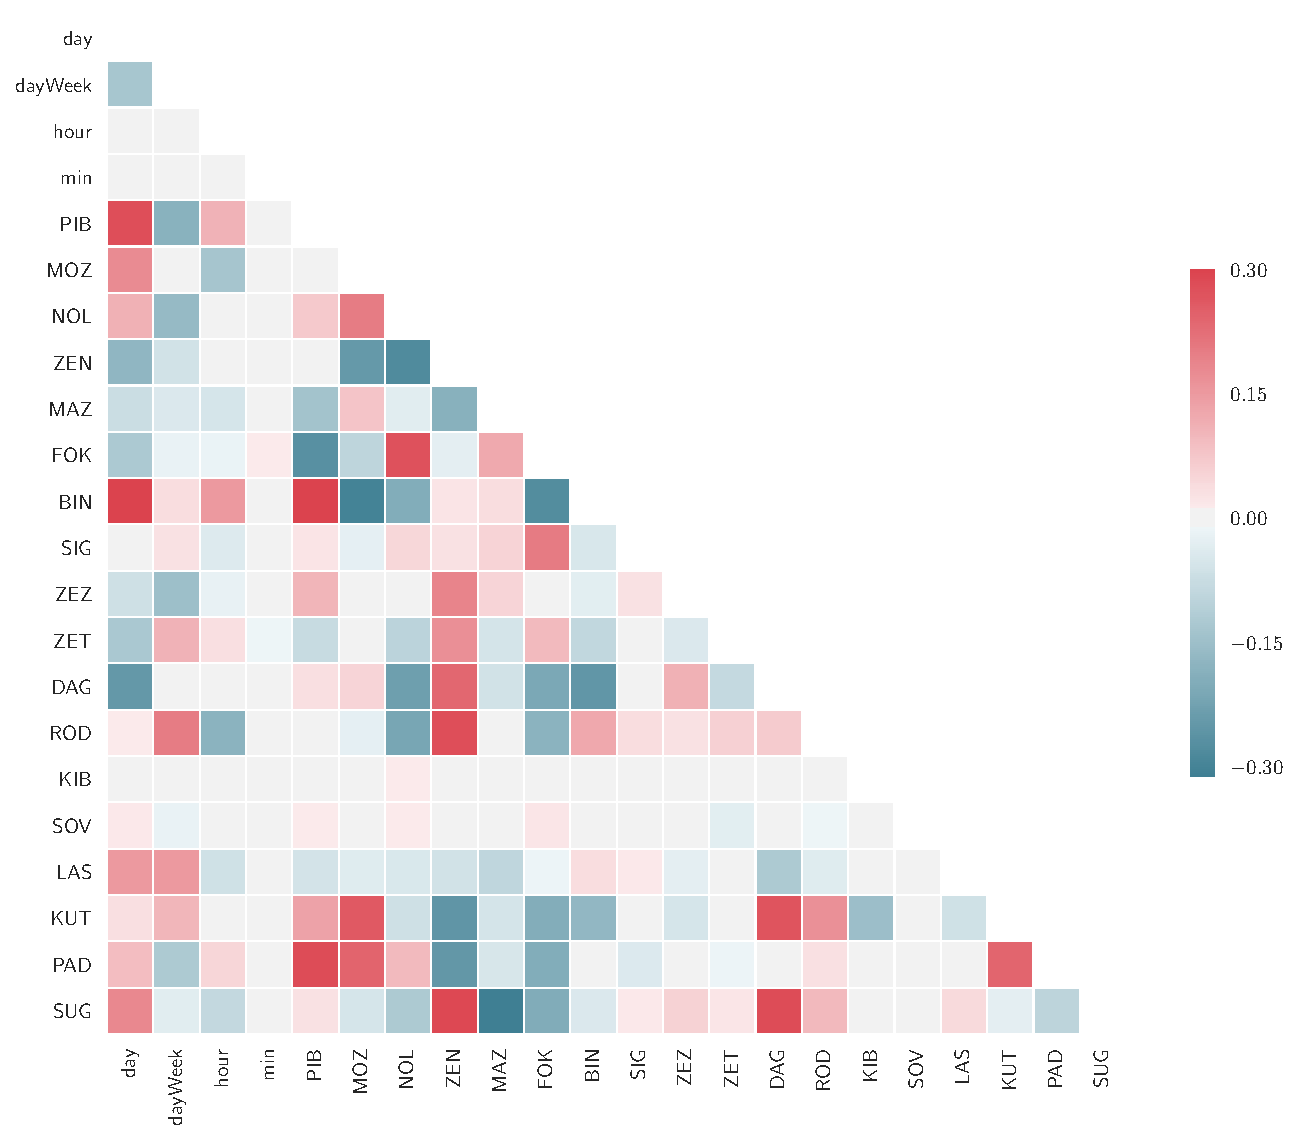
\includegraphics[width=0.8\linewidth]{correlation.pdf}
\captionof{figure}{Correlation matrix after removing correlated features with lower and upper bound threshold equal to -0.31, and 0.31 respectively}
\end{center}

\end{multicols}
}


%----------------------------------------------------------------------------------------
%	MATERIALS AND METHODS
%----------------------------------------------------------------------------------------

\headerbox{Training Pipeline}{name=training, row= 0, column=2, span = 2}{ % This block's bottom aligns with the bottom of the conclusion block
\tikzstyle{decision} = [diamond, draw, fill=blue!20, text width=4.5em, text badly centered, node distance=3cm, inner sep=0pt]
\tikzstyle{block} = [rectangle, draw, fill=blue!20, text width=7em, text centered, rounded corners, node distance=3cm, minimum height=4em]
\tikzstyle{line} = [draw, -latex' ]
\tikzstyle{cloud} = [draw, ellipse, fill=red!20, node distance=3cm, minimum height=2em]
\tikzstyle{block2} = [rectangle, draw, fill=blue!20, text width=8em, text centered, rounded corners, node distance=3cm, minimum height=6em]

\begin{tikzpicture}[node distance = 2cm, auto]
\node [block] (init) {Feature engineering \& correlation check};
\node [cloud, left of=init] (train) {Training data};
\node [block, below of=init] (drop) {feature drop};
\node [cloud, right of=init] (test) {Test data};
\node [block, below of=drop] (CV) {Cross-validation gridsearch};

\node [block, left of=drop] (imbData) {Imbalanced data};
\node [block, right of=CV] (balData) {Balanced data (via Oversampling)};
\path [line] (CV) -- (balData);
\path [line] (CV) -- (imbData);

\node [decision, below of=imbData] (svm) {Random Forest $-$ poor results };
\node [block, right of=balData] (rf) {Random Forest(RF) $-$ better results};
\path [line] (imbData) -- (svm);
\path [line] (balData) -- (rf);

\node [block, right of=rf] (rff) {RF using best hyperparameters};
\path [line] (rf) -- (rff);
\node [block2, above of=rff] (model) {split into oversampling(train), val, test};
\path [line] (rff) -- (model);

\node [block, left of=model] (trainmodel) {Train model and save};
\path [line] (model) -- (trainmodel);

\node [block, above of=trainmodel] (finalmodel) {Final model};
\path [line] (trainmodel) -- (finalmodel);

\path [line] (test) -- (finalmodel);

\node [decision, right of=finalmodel] (preds) {predictions in CSV};
\path [line] (finalmodel) -- (preds);

\path [line] (init) -- (drop);
\path [line] (drop) -- (CV);
\path [line, dashed] (train) -- (init);
\path [line, dashed] (test) -- (drop);
\path [line, dashed] (drop) -| (test);
\end{tikzpicture}
}


%----------------------------------------------------------------------------------------
%	Results
%----------------------------------------------------------------------------------------

\headerbox{Results}{name=results,column=2, span=2, below=training}{ % This block's bottom aligns with the bottom of the conclusion block

Donec faucibus purus at tortor egestas eu fermentum dolor facilisis. Maecenas tempor dui eu neque fringilla rutrum. Mauris \emph{lobortis} nisl accumsan.

\begin{center}
\begin{tabular}{l l l l l}
\toprule
\textbf{Model Type} & \textbf{Accuracy} & \textbf{Response 2} & \textbf{Response 2} & \textbf{Response 2}\\
\midrule
Imblanced 1 & 0.0003262 & 0.562  & 0.562  & 0.562 \\
Balanced 2 & 0.0015681 & 0.910  & 0.562  & 0.562 \\
\bottomrule
\end{tabular}
\captionof{table}{Table caption}
\end{center}
}
%----------------------------------------------------------------------------------------

%----------------------------------------------------------------------------------------
%	CONCLUSIONS
%----------------------------------------------------------------------------------------

\headerbox{Conclusions}{name=conclusions,column=2, span=2, below=results}{ % This block's bottom aligns with the bottom of the conclusion block

Donec faucibus purus at tortor egestas eu fermentum dolor facilisis. Maecenas tempor dui eu neque fringilla rutrum. Mauris \emph{lobortis} nisl accumsan.Donec faucibus purus at tortor egestas eu fermentum dolor facilisis. Maecenas tempor dui eu neque fringilla rutrum. Mauris \emph{lobortis} nisl accumsan.Donec faucibus purus at tortor egestas eu fermentum dolor facilisis. Maecenas tempor dui eu neque fringilla rutrum. Mauris \emph{lobortis} nisl accumsan.Donec faucibus purus at tortor egestas eu fermentum dolor facilisis. Maecenas tempor dui eu neque fringilla rutrum. Mauris \emph{lobortis} nisl accumsan.Donec faucibus purus at tortor egestas eu fermentum dolor facilisis. Maecenas tempor dui eu neque fringilla rutrum. Mauris \emph{lobortis} nisl accumsan.Donec faucibus purus at tortor egestas eu fermentum dolor facilisis. Maecenas tempor dui eu neque fringilla rutrum. Mauris \emph{lobortis} nisl accumsan.Donec faucibus purus at tortor egestas eu fermentum dolor facilisis. Maecenas tempor dui eu neque fringilla rutrum. Mauris \emph{lobortis} nisl accumsan.


}
%---



%
%%----------------------------------------------------------------------------------------
%%	REFERENCES
%%----------------------------------------------------------------------------------------
%
%\headerbox{References}{name=references,column=3,above=bottom}{
%
%\renewcommand{\section}[2]{\vskip 0.05em} % Get rid of the default "References" section title
%\nocite{*} % Insert publications even if they are not cited in the poster
%\small{ % Reduce the font size in this block
%\bibliographystyle{unsrt}
%\bibliography{sample} % Use sample.bib as the bibliography file
%}}



\end{poster}

\end{document}